\documentclass{article}
\usepackage{graphicx} % Required for inserting images
\usepackage[english]{babel}
\usepackage[utf8x]{inputenc}
\usepackage{amsmath}
\usepackage{amssymb}
\usepackage{float}
\usepackage[colorinlistoftodos]{todonotes}
\usepackage[authoryear]{natbib}
\usepackage{hyperref}
\usepackage{authblk}
\usepackage[margin=1in]{geometry}
\usepackage{pgfplots}
\usepackage{listings}
\usepackage{subfig}
\usepackage{multicol}
\usepackage{color}
\definecolor{listgray}{rgb}{0.88,0.88,0.88} 

\pgfplotsset{compat=1.12}

\lstset{
  language=Python,
  tabsize=2, 
  showspaces=false, 
  showstringspaces=false, 
  float=[htb], 
  captionpos=b, 
  basicstyle=\footnotesize, 
  % backgroundcolor=\color{listgray}, 
  % frame=tbrl, %t: top, r, b, l 
  % frameround=tttt, 
}

\title{
    Empirical Performance Analysis of AutoML Frameworks \\
    \large Project Report submitted as part of CS5999 Master of Engineering Project \\
    \large \textbf{Project Advisor: Prof. Sainyam Galhotra (sg@cs.cornell.edu) \footnote{Assistant Professor, Cornell University}}
    }
\author{Yogesh Eshwar Patil (yp445@cornell.edu) \footnote{CS MEng 2024, Cornell University}}
\date{December 2023}

\begin{document}

\maketitle

\begin{abstract}
Automated Machine Learning (AutoML) enables the automation of crucial machine learning (ML) steps such as data cleaning, feature engineering, model selection, and hyperparameter tuning. This project aims to evaluate the impact of clean data and noisy data on the performance of AutoML frameworks. The results help us show that additional data-cleaning techniques are essential even for the AutoML frameworks to be accurate. 
\end{abstract}

% \begin{multicols}{2}
\section{Introduction}
As more tasks in the industry are automated and demand machine learning solutions, the need for automating common tasks in the machine learning pipeline can prove to be extremely valuable. Such solutions when implemented responsibly, democratize the usage of artificial intelligence in a variety of applications, saving costs and time along with optimizing the workflows. \\
In this project, we evaluate the performance of two AutoML frameworks namely, \textbf{\href{https://autokeras.com/)}{AutoKeras}} and \textbf{\href{https://epistasislab.github.io/tpot/}{TPOT}} on text classification tasks. \footnote{Code implementations can be found on the GitHub \href{https://github.com/CornellDB/AutoMLDataPrep}{repository}}. We provide the same dataset as input to both frameworks and assess their performance using metrics such as precision, recall, and F1-score. With the help of this evaluation, we prove the need for additional cleaning of the dataset before it is fed into AutoML frameworks as input. Further, this also proves the need for the development of an efficient data-cleaning technique that co-exists and boosts AutoML performance. 

\section{Related Work}
Although AutoML frameworks are now generally available for use by the industry, they still demand the cleanest data possible to generate good predictions. \cite{literature1} describes the shifting of the approach from cleaning the data upstream before ML to cleaning the data for downstream ML. It examines the need for an end-to-end application-driven data-cleaning technique that works based on ML signals from the downstream model. It is based on the idea of applying data-cleaning solutions with respect to the problem being solved by the ML algorithm. While it is known that AutoML frameworks take significantly longer times on large-scale data, there is an interesting research by \cite{downsampling} which focusses on downsampling the data and its effects on the performance of a machine learning model.  \\
Several articles stress the need to data-cleaning tools as a precursor to AutoML frameworks. \cite{alphaclean} focused on developing automated data-cleaning pipeline generations that allow users with a rich collection of library features to define data quality measures. The search algorithm then sequences pipeline generation intending to maximize such user-defined measures. A similar tool for automated data cleaning in time-series data is cleanTS \cite{cleants} which also emphasizes the need for data cleaning and provides a complete R package. \cite{dataassist} also provides a pipeline for exploratory data analysis and data cleaning. 

\section{Implementation}

\subsection{Problem Definition and Dataset}
In this section, we provide a walkthrough of our setup for the experiments subsequently performed. We started with brainstorming ways of measuring the performance of different AutoML frameworks. We defined a problem statement that can be fed as an input. Our problem was to perform a binary text classification on textual input and examine the performance of AutoML frameworks. 

The two AutoML frameworks we discuss in this project are AutoKeras and TPOT. The Naive Bayes algorithm is also considered for benchmarking purposes. The dataset chosen for this task is the IMDB movie review \cite{imdbdata}  dataset. This dataset consists of 50,000 movie reviews classified as positive or negative sentiments.

\subsection{Introduction of Noise}
To measure how well the algorithms performed on clean data versus dirty data, we implemented an approach to introduce noise into the data. We explored adding Gaussian noise that is synthetic and reproducible, as well as realistic noise that is random and irreproducible. We discuss both approaches in the sections below.
\subsubsection{Gaussian Noise}
Gaussian noise is a type of random noise that follows Gaussian distribution. It is defined based on the mean and standard deviation provided and hence can be controlled. This type of noise resembles natural noise that occurs in nature. Below is the snippet of the code implemented to generate random noise. The noise is added to the text at the character level. 

\begin{lstlisting}[language=Python, caption=Gaussian Noise]
def add_gaussian_noise(text, mean=0, 
                       std_dev=0.1):
    """
    Add Gaussian noise to text.
    
    Parameters:
        text (str): The input text to 
        which noise will be added.
        mean (float): Mean of the 
        Gaussian distribution.
        std_dev (float): Standard 
        deviation of the Gaussian 
        distribution.
    
    Returns:
        str: The text with added 
        Gaussian noise.
    """
    noisy_text = list(text)
    
    # Generate Gaussian noise with 
    # the same length as the text
    noise = np.random.normal(mean, 
                        std_dev, 
                        len(noisy_text))
    
    for i in range(len(noisy_text)):
        noisy_text[i] = chr(
                    ord(noisy_text[i]) + 
                    int(noise[i]))
    
    return ''.join(noisy_text)
\end{lstlisting}

\subsubsection{Random Noise}
The (true) random noise approach was finalized as it is more realistic than other synthetic approaches discussed above. Since it is also random, there is no traceability or pattern that the model can potentially learn, leading to data leakage. Below is the snippet of the code implemented to generate random noise. 

\begin{lstlisting}[language=Python, caption=Random Noise]
def add_random_noise(text, noise_level):
    """
    Add random noise to text.
    Parameters:
        text (str): The input text to 
        which noise will be added.
        noise_level (int): Value between 
        0 and 1 signifying level of noise.
    Returns:
        str: The text with added random 
        noise.
    """
    noise_len = int(len(text) * 
                    noise_level)

    if noise_len == 0:
        return text
   
    noise_indices = random.sample(
        range(len(text)), noise_len)
   
    noisy_text = list(text)
 
    for idx in noise_indices:
        noisy_text[idx] = random.choice(
            string.ascii_letters)
    return ''.join(noisy_text)
\end{lstlisting}

\subsection{Preprocessing Data}
As part of data preprocessing, we first sampled data for various experiments depending on the time taken for pipeline generation by the AutoML frameworks. An important requirement for TPOT framework was to maintain the y-variable as \textbf{target}.

The reviews were also converted to binary form with $1$ as positive and $0$ as negative review. Then, the reviews were tokenized, checked for special characters, converted to lowercase, stopwords removed, and lemmatized. The tokens generated for each review were then embedded using Word2Vec embedding model. Further, an average word embedding was calculated for all the tokens in a sentence. 

The dataset was then split into training and testing splits in a $75:25$ ratio. Further, the data was converted to numpy arrays before being passed as input to AutoKeras framework's classifier.  
\section{Experiments}
With the data pipeline setup, the following experiments were performed and the performance of each technique was measured. There were six experiments conducted in total, three on clean data and three on noisy data.

\begin{table}[H]
    \centering
    \begin{tabular}{cccccc}
    \hline
        Experiments & Algorithm & Clean & Noise Type \\ \hline
        1 & Naive Bayes & Yes & N.A.\\ \hline
        2 & TPOT & Yes & N.A.\\ \hline
        3 & AutoKeras & Yes & N.A.\\ \hline
        4 & Naive Bayes & No & Random\\ \hline
        5 & TPOT & No & Random\\ \hline
        6 & AutoKeras & No & Random\\ \hline
    \end{tabular}
    \caption{Experiments}
    \label{tab:experiments}
\end{table}

Each of the experiments is recorded in the project repository in the form of notebooks and includes options to configure experiment parameters for multiple re-runs. The results obtained for the best selection of parameters after several experiment trials are described in the next section.  

\section {Results and Analysis}
In this section, we depict the results obtained based on the experiment trials conducted. The table and the charts below show the precision, recall, and F1-score plots for the six types of experiments.

\begin{table}[H]
    \centering
    \begin{tabular}{cccc}
    \hline
        Experiments & Precision & Recall & F1-Score \\ \hline
        Clean-NaiveBayes & $0.67$ & $0.70$ & $0.69$\\ \hline
        Clean-TPOT & $0.79$ & $0.81$ & $0.80$\\ \hline
        Clean-AutoKeras & $0.88$ & $0.83$ & $0.86$\\ \hline
        Noisy-NaiveBayes & $0.51$ & $0.97$ & $0.67$\\ \hline
        Noisy-TPOT & $0.56$ & $0.61$ & $0.58$\\ \hline
        Noisy-AutoKeras & $0.77$ & $0.77$ & $0.77$\\ \hline
    \end{tabular}
    \caption{Results}
    \label{tab:results}
\end{table}

\begin{figure*}
\begin{tabular}{ccc}
    \subfloat[Clean-NaiveBayes]{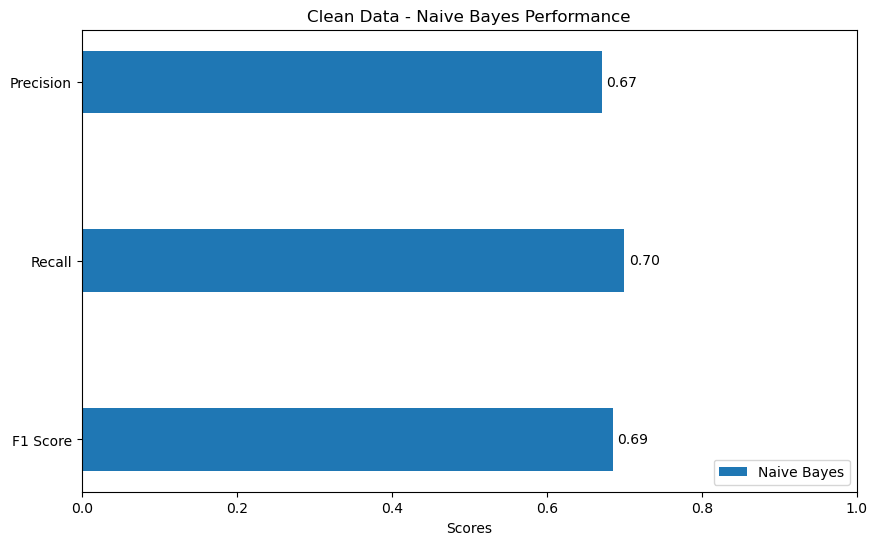
\includegraphics[width = 2in]{images/clean_nb.png}} &
    \subfloat[Clean-TPOT]{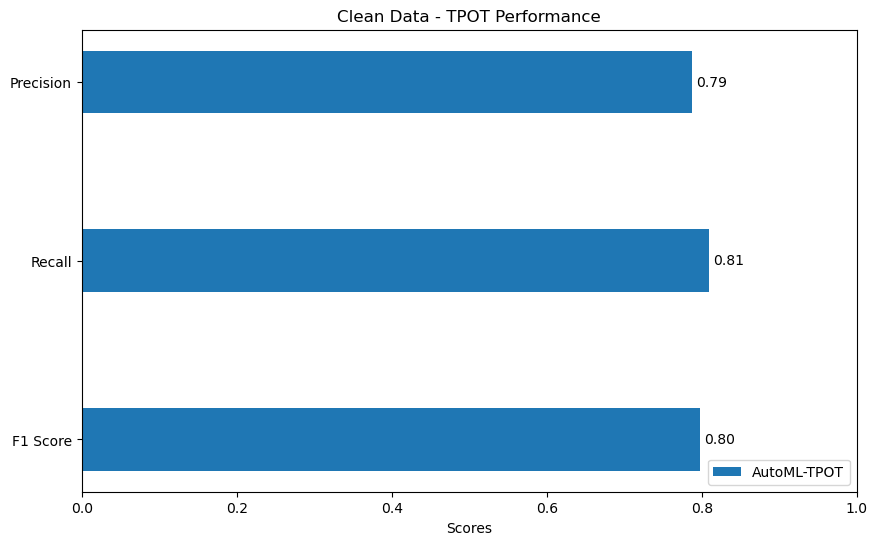
\includegraphics[width = 2in]{images/clean_tpot.png}} &
    \subfloat[Clean-AutoKeras]{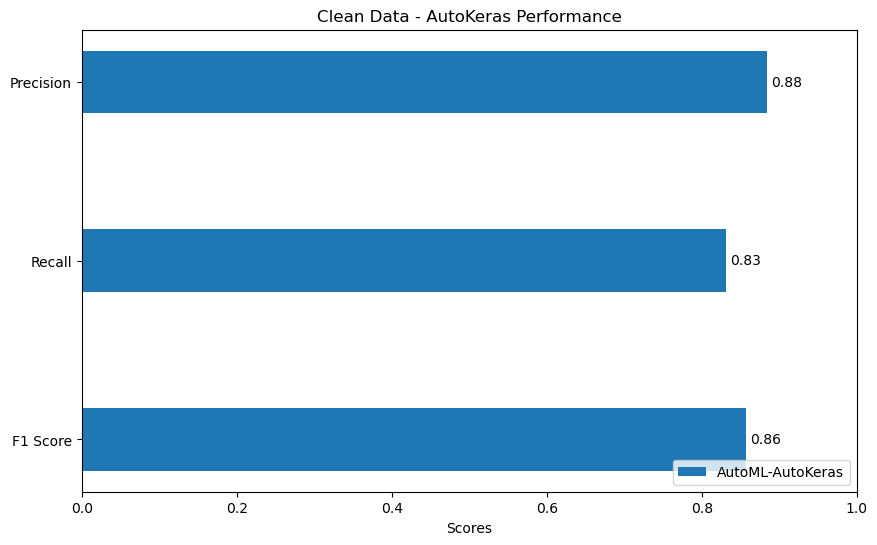
\includegraphics[width = 2in]{images/clean_ak.png}}\\
    \subfloat[Nosiy-NaiveBayes]{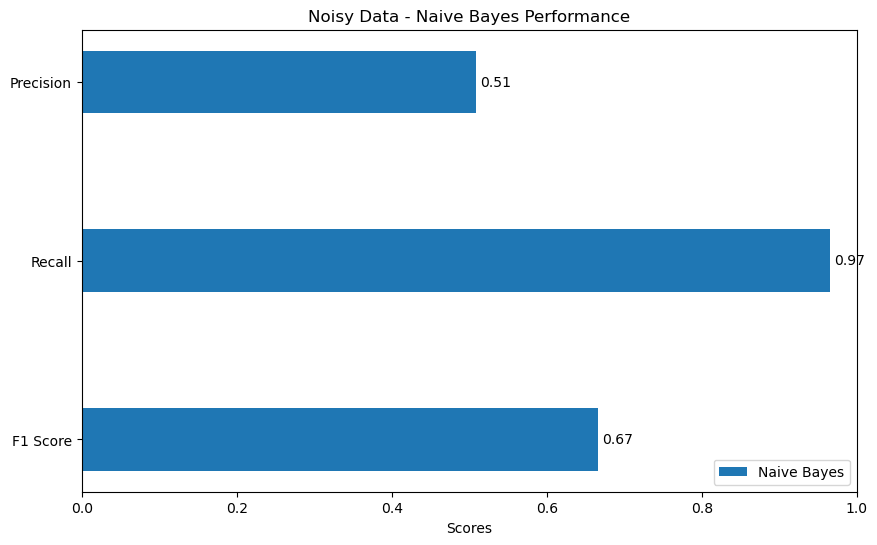
\includegraphics[width = 2in]{images/noisy_nb.png}} &
    \subfloat[Noisy-TPOT]{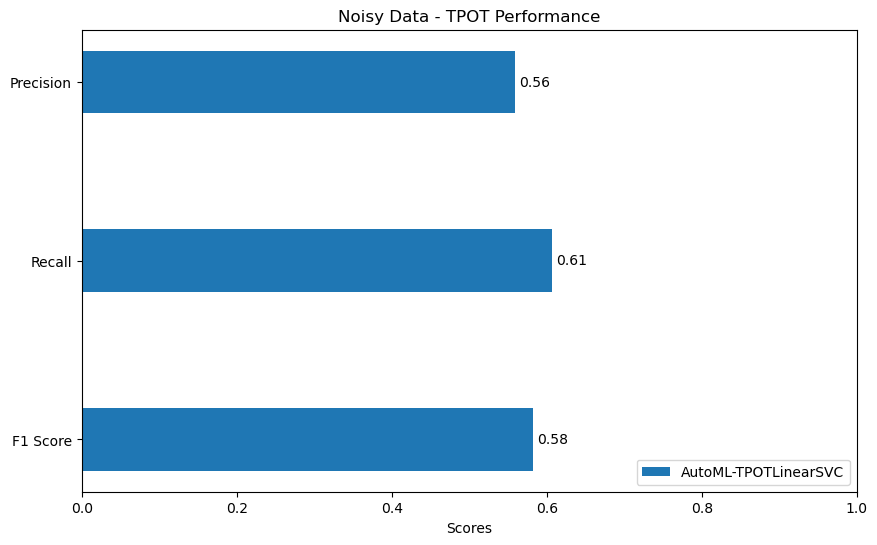
\includegraphics[width = 2in]{images/noisy_tpot.png}} &
    \subfloat[Noisy-AutoKeras]{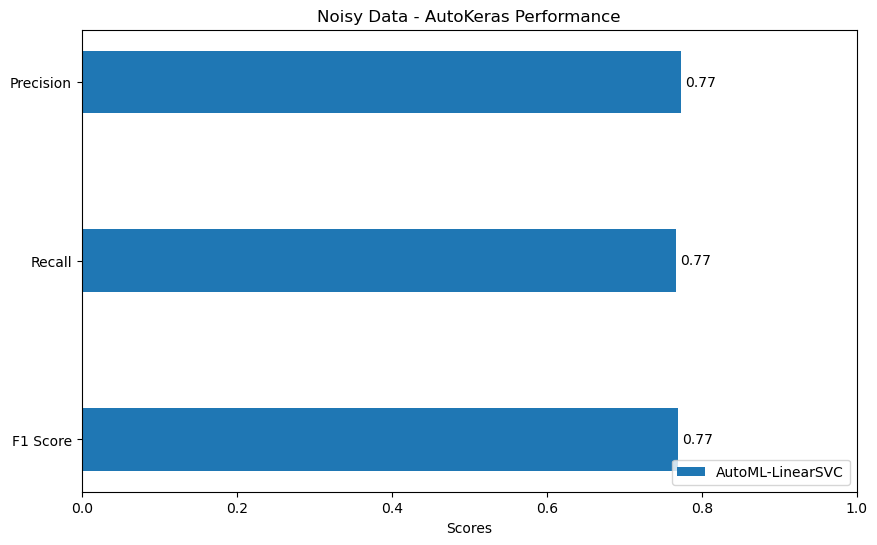
\includegraphics[width = 2in]{images/noisy_ak.png}}
\end{tabular}
    \caption{Results}
\end{figure*}

As can be seen in the results above, AutoKeras performs well compared to TPOT on the text classification task. The inherent ability to transform textual input into integer embeddings gives AutoKeras an advantage. The TPOT framework required us to manually embed the textual data using the Word2Vec model post-tokenization. A better and optimized manual embedding might prove to improve results on the TPOT. 

The results line up with our expectation that the noisy data requires additional data-cleaning steps before being fed into AutoML frameworks for improved accuracy. 

\section{Conclusion}
Our above experiments and their results prove the hypothesis that an additional data-cleaning technique is essential in the pipeline for AutoML frameworks to perform with better accuracy. In this project, we discussed the ongoing research on devising such automated data-cleaning techniques and brainstormed ways of improving the accuracy of AutoML. We implemented two approaches to introduce noise into the data for validating AutoML framework performances. We also then introduced Word2Vec embeddings required for specific frameworks such as TPOT. We obtained the results above based on six different types of experiments with multiple trials involving different parameter configurations. 

\section{Future Work}
This project opens up new opportunities for improvements and further development. The next course of action for this project could be multi-fold. 
\begin{enumerate}
    \item Implement a data-cleaning technique to manually clean the data before feeding the data as input into the chosen AutoML framework.
    \item Evaluate the performance of existing data-cleaning techniques such as \textit{alphaClean}, \textit{cleanTS}, and \textit{DataAssist} described above. 
    \item Evaluate the possibility of incorporating ML signal for auto-cleaning from the downstream application specific to the problem task.
\end{enumerate}

Continuation of research in this area would greatly benefit in democratizing artificially intelligent applications for many day-to-day industrial applications. While AutoML frameworks are evolving to enable automatic ML model selection, there is a parallel demand to improve the automated cleaning of data to best complement with existing frameworks and greatly improve accuracy. 

\bibliographystyle{apalike}
% \bibliographystyle{plain}
\bibliography{Bibliography}
% \end{multicols}

\clearpage

\end{document}
